\documentclass[a4paper,13pt]{report}

\usepackage[top=2.5cm,bottom=2.5cm,left=3cm,right=2cm]{geometry}
\usepackage[a4,frame,center]{crop}
\usepackage{graphicx}
\usepackage[english]{babel}
\usepackage[utf8]{inputenc}
\usepackage[T1]{fontenc}
\usepackage{ragged2e}
\usepackage{hyphenat}
\usepackage{lmodern}
\usepackage{fancyhdr}
\usepackage[toc,page]{appendix}
\usepackage{tabularx}
\usepackage{float}
\usepackage{amsmath}
\usepackage{indentfirst}
\usepackage[table]{xcolor}
\usepackage{array,multirow} 
\usepackage{varwidth}
\usepackage{listings}
\usepackage{background}
\usepackage{tikz}
\usepackage{hyperref}
\usetikzlibrary{calc}
\backgroundsetup{contents={}}
\setcounter{secnumdepth}{4}

\AtBeginDocument{%
\let\mtcontentsname\contentsname
\renewcommand\contentsname{\MakeUppercase\mtcontentsname}
}

\begin{document}
    \begin{titlepage}
        \centering
        \SetBgScale{1}
\SetBgAngle{0}
\SetBgColor{black}
\SetBgContents{
\begin{tikzpicture}[overlay,remember picture]
    \draw [line width=1pt,rounded corners=15pt,double]
        ($ (current page.north west) + (.5cm,-.5cm) $)
        rectangle
        ($ (current page.south east) + (-.5cm,.5cm) $);
\end{tikzpicture}
}
        \LARGE{\textsc{VIETNAM AVIATION ACADEMY}}\\
        \vspace{3mm}
        \normalsize{Department of Telecommunication - Electronics Engineering Technology} \\
        \vspace{3mm}
        \large{LOCATED IN HO CHI MINH CITY} \\
        \vspace{3mm}
        \includegraphics[scale=0.3]{img/logo.png} \\
        \vspace{3mm}
        \large{Graduation Thesis} \\
        \vspace{10mm}
        \huge{\textbf{"DROWSINESS DETECTION AND ALERT SYSTEM IN THE CAR"}} \\ 
        \vspace{20mm}
        \normalsize{Written by} \\ 
        \vspace{3mm}
        \large{\textbf{\textit{Nguyen Van Anh Tuan}}} \\ 
        \vspace{3mm}
        \large{\textbf{\textit{Roll.No.1753020018}}} \\ 
        \vspace{15mm}
        \large{Under the guidance of} \\
        \vspace{7mm}
        \centerline{\textbf{\large{Msc.Vo Phi Son}}} 
        \vspace{3.5cm}
        \centerline{\today}
    \end{titlepage}

    \newpage
    \thispagestyle{plain}
        \centering
        \LARGE{\textsc{VIETNAM AVIATION ACADEMY}}\\
        \vspace{3mm}
        \normalsize{Department of Telecommunication - Electronics Engineering Technology} \\
        \vspace{3mm}
        \large{LOCATED IN HO CHI MINH CITY} \\
        \vspace{3mm}
        \includegraphics[scale=0.3]{img/logo.png} \\
        \vspace{3mm}
        \large{Graduation Thesis} \\
        \vspace{15mm}
        \huge{\textbf{"DROWSINESS DETECTION AND ALERT SYSTEM IN THE CAR"}} \\ 
        \vspace{20mm}
        \normalsize{Written by} \\ 
        \vspace{3mm}
        \large{\textbf{\textit{Nguyen Van Anh Tuan}}} \\ 
        \vspace{3mm}
        \large{\textbf{\textit{Roll.No.1753020018}}} \\ 
        \vspace{15mm}
        \large{Under the guidance of} \\
        \vspace{7mm}
        \centerline{\textbf{\large{Msc.Vo Phi Son}}} 
        \vspace{3cm}
        \centerline{\today}
    
    \newpage
    \thispagestyle{plain}
    \centering
    \centerline{\textbf{\huge{PREAMBLE}}}
    \vspace{10mm}
    \begin{flushleft}
        In nowaday, along with the continuous development and progress of science and technology, image processing is 
        one of the topics that need attention and development. From the first researches about black-white image, 
        gray-scale and digital image, image processing has been studied deeply and applied a lot in our life. Beside that, 
        along with the development of Raspberry Pi with small scale, its promoting more development and application with 
        practice. \\ 
        \vspace{2mm}
        The application of Raspberry Pi in image processing aims to provide a few of image processing solutions to apply in 
        real life. In this project, i have used Raspberry Pi to detect drowsiness in the car with algorithms that can respond 
        in real time, the optimal solutions are simple but bring efficiency and high accuracy. I started to identify directly 
        through a camera connected to Raspberry Pi, and programmed using Python with the ability to track and mark the subject's 
        eyes, thereby determining whether the subject was closed or opened and alert a driver immediately, eyes are regconized by 
        the Facial Landmarks algorithm, then calculate the distance between the eyelids using Euclid to detect eye states and detect 
        drowsiness.
    \end{flushleft}
    \begin{flushright}
        \textbf{Auth.Nguyen Van Anh Tuan}
    \end{flushright}

    \newpage
    \thispagestyle{plain}
    \centering
    \centerline{\textbf{\huge{WORDS OF THANKS}}}
    \vspace{10mm}
    \begin{flushleft}
        Reality show that success is always associated with support of friends, teacher,... And i have special thanks to Mr.Vo Phi Son and my close friends 
        for helping me completing this project. \\ 
        \vspace{2mm}
        I have tried my best to do this project. However, due to my lack of experience and 
        knowledge, there are still some unexpected mistakes in the project. Please let me know your opinions and criticizes.
        Once again, thank you so much. 
    \end{flushleft}
    \begin{flushright}
        \textbf{Auth.Nguyen Van Anh Tuan}
    \end{flushright}

    \newpage
    \tableofcontents
    \listoffigures

    \chapter{OVERVIEW ABOUT PROJECT}

\renewcommand{\headrulewidth}{0.5pt}
\renewcommand{\footrulewidth}{0.5pt}
\thispagestyle{plain}
\pagestyle{fancy}
\fancyhf{}
\fancyhead[L]{\textbf{CHAPTER 1}}
\fancyhead[R]{\textbf{DROWSINESS DETECTION AND ALERT SYSTEM IN THE CAR}}
\raggedright
\fancyfoot[L]{From: Nguyen Van Anh Tuan}
\fancyfoot[R]{Page \thepage}

\justifying

\section{Introduction}
    Nowaday along with the strong development of Science Technology, Robot, Self-Driving Car, 
    AI,... In addition, image processing is a relatively new science compared to many other sciences, but now 
    it is one of the rapidly growing fields and attracts special attention from researchers, research centers, 
    application on this fascinating field. Image processing plays an important role in many practical applications 
    of science and technology as well as in everyday life such as: production and quality assurance, movement of robot, 
    self-driving car, guild tool for the blind, security and monitoring,... \\ 
    \vspace{3mm}
    Recently, the popularity and efficiency of using Raspberry Pi kit in applications in science and technology, 
    with characteristics like a miniature computer about the size of a mobile phone, runs an open operating system, 
    is equiped with a powerful processor, low power consumption, and low cost, allowing you to configure the Raspberry 
    Pi kit as a problem-solving computer. \\ 
    \vspace{3mm}
    Besides, from the actual needs, drowsiness while driving is quite common and it is also one of the casues of serious 
    accidents, requiring a device that can monitor the state of the person while driving to be able to promptly 
    warn the driver when the driver accidentally falls asleep while driving. \\ 
    \vspace{3mm}
    From these reasons has prompted me to research application of Raspberry Pi kit to image processing in order to offer 
    some image processing solutions that can be applied in life.

\section{Target and The Limits of Project}
    This project is the first step to learn about the application of processed images in reality, at the same time is also 
    a step to deploy the learned knowledge. Through research and serious work to practice manners, as well as perfecting 
    methods, researching thinking and solving a problem. With the objectives of the project is:
    \begin{itemize}
        \item Learning about Raspberry Pi 3 model B+ kit
        \item Install OS for Raspberry Pi 3 B+
        \item Learn about image processing
        \item Learn about OpenCV, Python
        \item Install library for OpenCV, Dlib
        \item Recognize techniques
        \item Drowsiness Detection by using camera connect to Raspberry Pi and alert to driver through speaker
        \item Write program
        \item Experimental model
        \item Write report
    \end{itemize}
    The limit of project is the distance from camera to object from 0,3-1m, detected object not to use glasses and 
    the angle is smaller than 40 degrees, if the object is out of this range, the detection maybe inaccurate or undetectable.

    \chapter{THEORETICAL BASIS}

\renewcommand{\headrulewidth}{0.5pt}
\renewcommand{\footrulewidth}{0.5pt}
\thispagestyle{plain}
\pagestyle{fancy}
\fancyhf{}
\fancyhead[L]{\textbf{CHAPTER 2}}
\fancyhead[R]{\textbf{DROWSINESS DETECTION AND ALERT SYSTEM IN THE CAR}}
\raggedright
\fancyfoot[L]{From: Nguyen Van Anh Tuan}
\fancyfoot[R]{Page \thepage}

\justifying

\section{Overview About Image Processing}
    \subsection{Introduction about Image Processing}
        Image processing is a method to perform some operations on an image, 
        in order to get an enhanced image or to extract some useful information from it. It is a type of signal 
        processing in which input is an image and output may be image or characteristics/features associated with 
        that image. Nowadays, image processing is among rapidly growing technologies. It forms core research area 
        within engineering and computer science disciplines too. \\ 
        \vspace{3mm}
        Image processing basically includes the following 3 steps:
        \begin{itemize}
            \item Importing the image via image acquisition tools
            \item Analysing and manipulating the image
            \item Output in which result can be altered image or report that is based on image analysis
        \end{itemize}
        There are two types of methods used for image processing namely, analogue and digital image processing. 
        Analog image processing can be used for the hard copies like printouts and photographs. Image analysts use 
        various fundamentals of interpretation while using these visual techniques. Digital image processing techniques 
        help in manipulation of the digital images by using computers. The three general phases that all types of data 
        have to undergo while using digital technique are pre-processing, enhancement, and display, information extraction.
        \begin{figure}[H]
            \centering
            \includegraphics[width=0.6\linewidth]{img/IP.jpg}
            \caption{Fundamental steps in digital processing}
        \end{figure}
        \subsubsection{Image Acquistion}
            This is the first step or process of the fundamental steps of digital image processing. Image acquisition could 
            be as simple as being given an image that is already in digital form. Generally, the image acquisition stage involves 
            preprocessing, such as scaling etc.
        \subsubsection{Image Enhancement}
            Image enhancement is among the simplest and most appealing areas of digital image processing. Basically, the idea behind 
            enhancement techniques is to bring out detail that is obscured, or simply to highlight certain features of interest in an 
            image. Such as, changing brightness \& contrast etc.
        \subsubsection{Image Restoration}
            Image restoration is an area that also deals with improving the appearance of an image. However, unlike enhancement, 
            which is subjective, image restoration is objective, in the sense that restoration techniques tend to be based on mathematical 
            or probabilistic models of image degradation.
        \subsubsection{Color Image Processing}
            Color image processing is an area that has been gaining its importance because of the significant increase in the use of digital 
            images over the Internet. This may include color modeling and processing in a digital domain etc.
        \subsubsection{Wavelets and Multiresolution Processing}
            Wavelets are the foundation for representing images in various degrees of resolution. Images subdivision successively into smaller 
            regions for data compression and for pyramidal representation.
        \subsubsection{Compression}
            Compression deals with techniques for reducing the storage required to save an image or the bandwidth to transmit it. Particularly in 
            the uses of internet it is very much necessary to compress data.
        \subsubsection{Morphological Processing}
            Morphological processing deals with tools for extracting image components that are useful in the representation and description of shape.
        \subsubsection{Segmentation}
            Segmentation procedures partition an image into its constituent parts or objects. In general, autonomous segmentation is one of the most difficult 
            tasks in digital image processing. A rugged segmentation procedure brings the process a long way toward successful solution of imaging problems that 
            require objects to be identified individually.
        \subsubsection{Representation and Description}
            Representation and description almost always follow the output of a segmentation stage, which usually is raw pixel data, constituting either the boundary 
            of a region or all the points in the region itself. Choosing a representation is only part of the solution for transforming raw data into a form suitable 
            for subsequent computer processing. Description deals with extracting attributes that result in some quantitative information of interest or are basic for 
            differentiating one class of objects from another.
        \subsubsection{Object Recognition}
            Recognition is the process that assigns a label, such as, “vehicle” to an object based on its descriptors.
        \subsubsection{Knowledge Base}
            Knowledge may be as simple as detailing regions of an image where the information of interest is known to be located, thus limiting the search that has to be 
            conducted in seeking that information. The knowledge base also can be quite complex, such as an interrelated list of all major possible defects in a materials 
            inspection problem or an image database containing high-resolution satellite images of a region in connection with change-detection applications.
    \subsection{The Components of Image Processing}
        \subsubsection{Digital Image}
            A digital image is a finite set of pixels with a gray level suitable for describing an image close to the real image. The number of pixels 
            determines the resolution of the image. The higher quality of the image, the more clearly the image's points are displayed, making the image 
            more realistic and sharp.
        \subsubsection{Picture Element}
            In digital imaging, pixel, pel, or picture element is a smallest addressable element in a raster image, or the smallest addressable element in an \textbf{all points 
            addressable display device}; so it is the smallest controllable element of a picture represented on the screen. \\ 
            \vspace{3mm}
            Each pixel is a sample of an original image; more samples typically provide more accurate representations of the original. The intensity of each pixel is variable. 
            In color imaging systems, a color is typically represented by three or four component intensities such as red, green, and blue, or cyan, magenta, yellow, and black. \\ 
            \vspace{3mm}
            In some contexts (such as descriptions of \textbf{camera sensors}), pixel refers to a single scalar element of a multi-component representation (called a photosite in the 
            camera sensor context, although sensel is sometimes used), while in yet other contexts it may refer to the set of component intensities for a spatial position.
            \begin{figure}[H]
                \centering
                \includegraphics[width=0.6\linewidth]{img/Pixel-example.png}
                \caption{Pixel example}
            \end{figure}
            Pixel is an element of digital image at coordinate (x,y) with gray level or certain color. The size and the distance between those pixels are chosen appropriately so that 
            the human eye perceives spatial continuity and gray level (or color) of digital image like real image. Each of element in matrix is called an image element.
        \subsubsection{Gray Level of Picture}
            Gray level is the result of conversion of 1 luminosity value of 1 pixel positive integer value. Usually identified in [0,255] depending on the value each pixel is 
            represented. Common gray scale values is: 16, 32, 64, 128, 256 (level 256 is universal level). The reason is computer techniques use 1 byte (8 bits) to represent 
            the gray level. Gray level use 1 byte represent: 28 = level 256, it mean from 0 to 255).
            \begin{figure}[H]
                \centering
                \includegraphics[width=0.6\linewidth]{img/gray-scale.png}
                \caption{Gray scale image example}
            \end{figure}
        \subsubsection{Image Resolution}
            Image resolution is detail an image holds. The term applies to raster digital images, film images, and other types of images. Higher resolution means more image detail. \\ 
            \vspace{3mm}
            Image resolution can be measured in various ways. Resolution quantifies how close lines can be to each other and still be visibly resolved. Resolution units can be tied 
            to physical sizes (e.g. lines per mm, lines per inch), to the overall size of a picture (lines per picture height, also knnown simply as lines, TV lines, or TVL), 
            or to angular subtense. Line pairs are often used instead of lines; a line pair comprises a dark line and an adjacent light line. A line is either a dark line or 
            a light line. A resolution of 10 lines per milimeter means 5 dark line alternating with 5 light lines, or 5 line pairs per milimeter (5 LP/mm). Photographic lens and film 
            resolution are most often quoted in line pairs per milimeter. \\ 
            \vspace{3mm}
            For example: Image resolution in CGA display (Color Graphic Adaptor) is a grid of points across the screen: 320 vertical points * 200 image points (320*200).
            Obviously, with the same CGA display 12 inches we notice smoother than the screen CGA 17 inches with resolution is 320*200. The reason is with the same resolution but 
            the larger the screen area, the less smooth.
        \subsubsection{Types of image classification}
            \begin{itemize}
                \item \textbf{Binary Image:} is one that consists of pixels that can have one of exactly two colors, usually black and white. Binary images are also called bi-level 
                or two-level, Pixelart made of two colours is often referred to as 1-Bit or 1bit. This means that each pixel is stored as a single bit—i.e., a 0 or 1. \\
                \vspace{2mm}
                The names black-and-white, B\&W, monochrome or monochromatic are often used for this concept, but may also designate any images that have only one sample per pixel, 
                such as grayscale images. In Photoshop parlance, a binary image is the same as an image in "Bitmap" mode. \\ 
                \vspace{2mm}
                Binary images often arise in digital image processing as masks or thresholding, and dithering. Some input/output devices, such as laser printers, fax machines, 
                and bilevel computer displays, can only handle bilevel images. \\ 
                \vspace{2mm}
                A binary image can be stored in memory as a bitmap, a packed array of bits. A 640×480 image requires 37.5 KiB of storage. Because of the small size of the image files, 
                fax machine and document management solutions usually use this format. Most binary images also compress well with simple run-length compression schemes. \\ 
                \vspace{2mm}
                Binary images can be interpreted as subsets of the two-dimensional integer lattice $Z^2$; the field of morphological image processing was largely inspired by this view.
                \item \textbf{RGB Image:} RGB Color Model is an additive color model, in which red, green, and blue light are added together in various ways to reproduce a broad array 
                of colors. The name of the model comes from the initials of the three additive primary colors, red, green, and blue. \\ 
                \vspace{2mm}
                RGB is a device-dependent color model: different devices detect or reproduce a given RGB value differently, since the color elements (such as phosphors or dyes) 
                and their response to the individual R, G, and B levels vary from manufacturer to manufacturer, or even in the same device over time. Thus an RGB value does not define 
                the same color across devices without some kind of color management.
                \begin{figure}[H]
                    \centering
                    \includegraphics[width=0.6\linewidth]{img/RGB.png}
                    \caption{Additive color mixing}
                \end{figure}
                The choice of primary colors is related to the physiology of the human eye; good primaries are stimuli that maximize the difference between the responses of the cone 
                cells of the human retina to light of different wavelengths, and that thereby make a large color triangle. \\ 
                \vspace{2mm}
                The normal three kinds of light-sensitive photoreceptor cells in the human eye (cone cells) respond most to yellow (long wavelength or L), green (medium or M), 
                and violet (short or S) light (peak wavelengths near 570 nm, 540 nm and 440 nm, respectively). The difference in the signals received from the three kinds allows 
                the brain to differentiate a wide gamut of different colors, while being most sensitive (overall) to yellowish-green light and to differences between hues in the 
                green-to-orange region.
                \begin{figure}[H]
                    \centering
                    \includegraphics[width=0.6\linewidth]{img/primary-color.png}
                    \caption{A set of primary colors, such as the sRGB primaries, define a color triangle}
                \end{figure}
                \item \textbf{Image Transformation:} is a function. A function that maps one set to another set after performing some operations. \\ 
                \vspace{2mm}
                Image transformation is consider this equation:
                \begin{align}
                    G(x,y) = T{f(x,y)}
                \end{align}
                In this equation, $F(x,y)$ is input image on which transformation function has to be applied; $G(x,y)$ is the output image or processed image; $T$ is the transformation 
                function. This relation between input image and the processed output image can also be represented as: $s = T(r)$ where $r$ is actually the pixel value or gray level intensity 
                of $f(x,y)$ at any point. And $s$ is the pixel value or gray level intensity of $g(x,y)$ at any point. \\
                \vspace{2mm}
                The basic gray level transformation has been discussed in our tutorial of basic gray level transformations. There is some image transformations like: \texttt{Fourier Transform, Cousin, 
                Sin, convolution transform, Kronecker product}.
            \end{itemize}
    \subsection{Parts of The Image Processing System}
        \begin{figure}[H]
            \centering
            \includegraphics[width=0.6\linewidth]{img/Drowsiness.png}
            \caption{The part of image processing system}
        \end{figure}
        \textbf{Image Receiver Department} is usually a camera, scaners, image sensor,... In this project, a pi camera with 5mpx resolution is used to capture images. \\ 
        \vspace{3mm}
        \textbf{Image Processing Department} is specialized processing equipment or computers,... Specifically here using a Raspberry pi 3B + computer for image processing. \\ 
        \vspace{3mm}
        \textbf{Integrated Development Environment} using Thony Python IDE software to write program. \\ 
        \vspace{3mm}
        \textbf{Warning Devices} speaker alarms.

\section{Face Regconition Algorithm}
    Before we go to the algorithms for face detection we should understand how to detect a face even though we don't know who the subject is. \\
    \vspace{3mm}
    Face Recognition is a way of recognizing a human face through technology. A facial recognition system uses biometrics to map facial features from a photograph or video. 
    It compares the information with a database of known faces to find a match. Facial recognition can help verify personal identity, but it also raises privacy issues. \\ 
    \vspace{3mm}
    The recognition of a face in a video sequence is split into three primary tasks: Face Detection, Face Prediction, and Face Tracking. The tasks performed in the Face Capture 
    program are performed during face recognition as well. To recognize the face obtained, a vector of HOG features of the face is extracted. This vector is then used in the SVM 
    model to determine a matching score for the input vector with each of the labels. The SVM returns the label with the maximum score, which represents the confidence to the 
    closest match within the trained face data. 
    \begin{figure}[H]
        \centering
        \includegraphics[width=0.6\linewidth]{img/face-recognition.jpg}
        \caption{Block diagram of the face recognition process}
    \end{figure}
    The task of calculating matching scores is exceptionally heavy to compute. Hence, once detected and identified, the labeled face in an image needs to be tracked to reduce the 
    computation in future frames until the face eventually disappears from the video. Of all the available trackers, the Camshift tracking algorithm is used since it produces the 
    best results with faces. \\ 
    \vspace{3mm}
    Where you see a face, recognition technology sees data. That data can be stored and accessed. 
    For instance, half of all American adults have their images stored in one or more facial-recognition databases that law enforcement agencies can search, according to a 
    Georgetown University study. Technologies can be different, but there are the basic steps:
    \begin{itemize}
        \item \textbf{Step 1.} A picture of your face is captured from a photo or video. Your face might appear alone or in a crowd. Your image may show you looking straight 
        ahead or nearly in profile
        \item \textbf{Step 2.} Facial recognition software reads the geometry of your face. Key factors include the distance between your eyes and the distance from forehead to chin. 
        The software identifies facial landmarks — one system identifies 68 of them — that are key to distinguishing your face. The result: your facial signature
        \item \textbf{Step 3.} Your facial signature — a mathematical formula — is compared to a database of known faces. And consider this: at least 117 million Americans have images 
        of their faces in one or more police databases. According to a May 2018 report, the FBI has had access to 412 million facial images for searches
        \item \textbf{Step 4.} A determination is made. Your faceprint may match that of an image in a facial recognition system database.
    \end{itemize}
    The gist of the pipeline can be seen in figure down here: 
    \begin{figure}[H]
        \centering
        \includegraphics[width=0.6\linewidth]{img/opencv.jpg}
        \caption{An overview of the OpenCV face recognition pipeline}
    \end{figure}
    First, we input an image or video frame to our face recognition pipeline. Given the input image, we apply face detection to detect the location of a face in the image. Optionally 
    we can compute \textbf{Facial Landmarks}, enabling us to \textbf{Preprocess and align the face}. \\ 
    \vspace{3mm}
    Face alignment, as the name suggests, is the process of identifying the geometric structure of the faces and attempting to obtain a canonical alignment of the face based on translation, 
    rotation, and scale. While optional, face alignment has been demonstrated to increase face recognition accuracy in some pipelines. After we’ve (optionally) applied face alignment 
    and cropping, we pass the input face through our deep neural network:
    \begin{figure}[H]
        \centering
        \includegraphics[width=0.6\linewidth]{img/pyimgsearch.png}
        \caption{How the deep learning face recognition model computes the face embedding}
    \end{figure}
    The FaceNet deep learning model computes a 128-d embedding that quantifies the face itself. But how does the network actually compute the face embedding? The answer lies in the training 
    process itself, including:
    \begin{itemize}
        \item The input data to the network
        \item The triplet loss function
    \end{itemize}
    To train a face recognition model with deep learning, each input batch of data includes three images:
    \begin{itemize}
        \item The anchor
        \item The positive image
        \item The negative image
    \end{itemize}
    The anchor is our current face and has identity A. \\ 
    \vspace{3mm}
    The second image is our positive image — this image also contains a face of person A. \\ 
    \vspace{3mm}
    The negative image, on the other hand, does not have the same identity, and could belong to person B, C, or even Y! \\
    \vspace{3mm}
    The point is that the anchor and positive image both belong to the same person/face while the negative image does not contain the same face. The neural network computes the 128-d 
    embeddings for each face and then tweaks the weights of the network (via the triplet loss function) such that:
    \begin{itemize}
        \item The 128-d embeddings of the anchor and positive image lie closer together
        \item While at the same time, pushing the embeddings for the negative image father away
    \end{itemize}
    In this manner, the network is able to learn to quantify faces and return highly robust and discriminating embeddings suitable for face recognition.

    \subsection{Face Detection using HOG}
        The essential thought behind the histogram of oriented gradients descriptor is that local object appearance and shape within an image can be described by the distribution of intensity gradients or edge directions. 
        The image is divided into small connected regions called cells, and for the pixels within each cell, a histogram of gradient directions is compiled. The descriptor is the concatenation of these histograms. For 
        improved accuracy, the local histograms can be contrast-normalized by calculating a measure of the intensity across a larger region of the image, called a block, and then using this value to normalize all cells 
        within the block. This normalization results in better invariance to changes in illumination and shadowing. \\
        \vspace{3mm}
        In the current example, all the face sample images of a person are fed to the feature descriptor extraction algorithm; i.e., a HOG. The descriptors are gradient vectors generated per pixel of the image. 
        The gradient for each pixel consists of magnitude and direction, calculated using the following formular:
        \begin{figure}[H]
            \centering
            \includegraphics[width=0.6\linewidth]{img/HOG-feature.jpg}
            \caption{HOG features sample face}
        \end{figure}
        \begin{align}
            g = \sqrt{g^2_x + g^2_y} \\ 
            \theta = \arctan{\frac{g_y}{g_x}}
        \end{align}
        Gx and Gy are respectively the horizontal and vertical components of the change in the pixel intensity. A window size of 128 x 144 is used for face images since it matches the general aspect ratio of human faces. 
        The descriptors are calculated over blocks of pixels with 8 x 8 dimensions. These descriptor values for each pixel over 8 x 8 block are quantized into 9 bins, where each bin represents a directional angle of gradient 
        and value in that bin, which is the summation of the magnitudes of all pixels with the same angle. \\ 
        \vspace{3mm}
        Further, the histogram is then normalized over a 16 x 16 block size, which means four blocks of 8 x 8 are normalized together to minimize light conditions. This mechanism mitigates the accuracy drop due to a 
        change in light. The SVM model is trained using a number of HOG vectors for multiple faces. \\
        \vspace{3mm}
        There is some review entire detailed process of training an object detector using Histogram Oriented Gradients, each step can be fairly detailed. It goes like something like this:
        \begin{itemize}
            \item \textbf{Step 1:} Sample P positive samples from your training data of the object(s) you want to detect and extract HOG descriptors from these samples;
            \item \textbf{Step 2:} Sample N negative samples from a negative training set that \textbf{does not contain} any of the objects you want to detect and extract HOG descriptors from these samples as well. In practice N $\gg$ P;
            \item \textbf{Step 3:} Train a Linear Support Vector Machine on your positive and negative samples;
            \item \textbf{Step 4:} 
                \begin{figure}[H]
                    \centering
                    \includegraphics[width=0.6\linewidth]{img/sliding_window_example.jpg}
                    \caption{Example of the sliding a window approach, where we slide a window from left-to-right and top-to-bottom}
                \end{figure}
                \textbf{Apply hard-negative mining}, For each image and each possible scale of each image in your negative training set, apply the sliding window technique and slide your window across the image. 
                At each window compute your HOG descriptors and apply your classifier. If your classifier (incorrectly) classifies a given window as an object (and it will, there will absolutely be false-positives), 
                record the feature vector associated with the false-positive patch along with the probability of the classification. \textbf{This approach is called hard-negative mining}.
            \item \textbf{Step 5:} Take the false-positive samples found during the hard-negative mining stage, sort them by their confidence (i.e. probability) and re-train your classifier using these hard-negative samples.
            \item \textbf{Step 6:} Your classifier is now trained and can be applied to your test dataset. Again, just like in Step 4, for each image in your test set, and for each scale of the image, apply the sliding window technique. 
                At each window extract HOG descriptors and apply your classifier. If your classifier detects an object with sufficiently large probability, record the bounding box of the window. After you have finished scanning the image, 
                apply non-maximum suppression to remove redundant and overlapping bounding boxes. \\ 
                \vspace{2mm}
                These are the bare minimum steps required, but by using this 6-step process you can train and build object detection classifiers of your own! Extensions to this approach include a deformable parts model and Exemplar SVMs, 
                where you train a classifier for each positive instance rather than a collection of them. \\ 
                \vspace{2mm}
                However, if you’ve ever worked with object detection in images you’ve likely ran into the problem of detecting multiple bounding boxes around the object you want to detect in the image. And here’s an example of this overlapping bounding box problem:
                \begin{figure}[H]
                    \centering
                    \includegraphics[width=0.6\linewidth]{img/multiple-overlapping.jpg}
                    \caption{(Left) Detecting multiple overlapping bounding boxes around the face we want to detect. (Right) Applying non-maximum suppression to remove the redundant bounding boxes.}
                \end{figure}
        \end{itemize}

    \subsection{Haar-like Feature (Haar-Cascade)}
        \subsubsection{Theory}
            Object Detection using Haar feature-based cascade classifiers is an effective object detection method is a machine learning based approach where a cascade function is trained from a lot of positive and negative images. It is then used to detect objects in other images. \\ 
            \vspace{3mm}
            Here we will work with face detection. Initially, the algorithm needs a lot of positive images (images of faces) and negative images (images without faces) to train the classifier. Then we need to extract features from it. For this, Haar features shown in the below image 
            are used. They are just like our convolutional kernel. Each feature is a single value obtained by subtracting sum of pixels under the white rectangle from sum of pixels under the black rectangle.
            \begin{figure}[H]
                \centering
                \includegraphics[width=0.6\linewidth]{img/haar_features.jpg}
                \caption{Feature 4 rectangle}
            \end{figure}
            \begin{figure}[H]
                \centering
                \includegraphics[width=0.6\linewidth]{img/feature_center.png}
                \caption{Feature in center}
            \end{figure}
            Using above features, we can calculate the value of the Haar-Like feature as the difference between the sum of the pixels of the black area and the white area as shown in the following formula:
            \begin{align}
                F(x) = Sum of black area - Sum of white area (gray level of pixel)
            \end{align} 
            There is a concept called \textbf{"Integral Image"}, is the 2D array with the size equal to the size of the image to be Haar-Like feature, with each element of this array is computed by summing the pixels above and left of it.
        \subsubsection{Integral Image}
            The idea of this concept is transforming an input images into a summed-area table, where the value at any point (x, y) in that table is the sum of all the pixels above and to the left of (x, y), inclusive:
            \begin{align}
                P(x,y) = \displaystyle\sum_{x' \leq x, y' \leq y} i(x',y')
            \end{align}
            Where I(x,y) is the value of the integral image pixel in the position (x,y), while i(x,y) is the corresponding intensity in the original image. It is a recursive formula, hence, if we start from one corner of the input image, we will have the same result in the integral image. 
            To make it clearer, let’s see an example:
            \begin{figure}[H]
                \centering
                \includegraphics[width=0.6\linewidth]{img/example_integral.png}
                \caption{Example of Integral Image}
            \end{figure}
            In this figure we added one row and column of zeros, since we need one step backward in order to start the recursive formula. Hence, if your image is $w$ pixels wide and $h$ pixels high, then the integral of this will be $w+1$ pixels wide and $h+1$ pixels high. \\ 
            \vspace{3mm}
            Moving to the computations, let's start from the first pixel in the original image with intensity 1: the integral image returns exactly the same value, since it is computing (1+0+0). Then, pixel '3' becomes '4', since it is 3+1+0+0. With the same procedure, we obtain an 
            "8" (7+1+0) and a '20' (9+3+1+7). \\ 
            \vspace{3mm}
            We have a new image, but how is supposed to be useful? The answer rely in an unique property of the integral image. Indeed, it turned our that if you need to compute the summation within a window in the input image, hence that summation is equal to a linear combination 
            of the corresponding window’s corner in the integral image, as follows:
            \begin{align}
                \Sigma_{x_0 < x < x_1; y_0 < y < y_1} i(x,y) = I(D) + I(A) - I(B) - I(C)
            \end{align}
            Where is $A,B,C$ and $D$ are the corners of the corresponding window in the integral image.
            \begin{figure}[H]
                \centering
                \includegraphics[width=0.6\linewidth]{img/corners_corresponding.png}
                \caption{Integral Image Approach}
            \end{figure}
            This reduces the number of computations by far. To give you an idea, consider a 100×100 image with a 9×9 window. We want to compute the sum of the pixel intensities within that window, which requires 8 operations. If we repeat this procedure 100 times, we obtain 800 operations. \\
            \vspace{3mm}
            Now let’s see the integral image approach. First, we compute the summed-area table, which requires 56 operations. Then, considering the same 9×9 window, to compute the sum of pixel intensity we just need the above formula, which is made of 3 operations. Hence, the total number 
            of operations is 56+3*100=356. As you can see, it is less than a half. \\
            \vspace{3mm}
            This procedure is widely used in computer vision and Haar Cascade algorithm is based exactly on that. \\
            \vspace{3mm}
            The idea is passing these filters on the image, inspecting one portion (or window) at the time. Then, for each window, all the pixel intensities of, respectively, white and black portions are summed. Finally, the value obtained by subtracting those two summations is the value 
            of the feature extracted. Ideally, a great value of a feature means it is relevant. Namely, if we consider the Edge feature and apply it to the following Black and White pic:
            \begin{figure}[H]
                \centering
                \includegraphics[width=0.6\linewidth]{img/Emma.png}
                \caption{Black and White picture}
            \end{figure}
            We will obtain a significant value, hence the algorithm will return an edge feature with high probability. Of course, the real intensities of pixels is never equal to white or black, and we will often face a similar situation:
            \begin{figure}[H]
                \centering
                \includegraphics[width=0.6\linewidth]{img/real_pixel.png}
                \caption{The real intensities of pixels}
            \end{figure}
            Nevertheless, the idea remains the same: the higher the result (that is, the difference between black and white summations), the higher the probability of that window of being a relevant feature. \\ 
            \vspace{3mm}
            Imagine that the huge amount of features returned by this computation. To give you an idea, even a 24x24 window results over 160000 features, and windows within an image are a lot. How to make this process more efficient? The solution came out with the concept of Summed-area table, 
            also known as Integral Image. It is a data structure and algorithm for generating the sum of values in a rectangular subset of a grid. The goal is reducing the number of computations needed to obtain the summations of pixel intensities within a window. \\
            \vspace{3mm}
            Next is also involves efficiency and optimization. Besides being numerous, features might also be irrelevant. Among the features we obtain (that are more than 160000), how can we decide which ones are good? The answer to this question relies on the concept of Ensembilg method: 
            by combining many algorithms, weak by definition, we can create a strong algorithm. This is accomplished using \textbf{Adaboost} which both selects the best features and trains the classifiers that use them. This algorithm constructs a “strong” classifier as a linear combination of weighted 
            simple “weak” classifiers. \\ 
            \vspace{3mm}
            The last concept which needs to be introduced is a final element of optimization (in terms of the time of training). Indeed, even though we reduced our 160000+ features to a more manageable number, the latter is still high: applying all the features on all the windows will take a lot of time. 
            That’s why we use the concept of Cascade of classifiers: instead of applying all the features on a window, it groups the features into different stages of classifiers and applies one-by-one. If a window fails (the difference between white and black summations is low) the first stage (which normally 
            includes few features), the algorithm discards it: it won’t consider remaining features on it. If it passes, the algorithm applies the second stage of features and continues the process.

    \subsection{AdaBoost Algorithm}
        In recent years, boosting algorithms gained massive popularity in data science or machine learning competitions. Most of the winners of these competitions use boosting algorithms to achieve high accuracy. These Data science competitions provide 
        the global platform for learning, exploring and providing solutions for various business and government problems. Boosting algorithms combine multiple low accuracy(or weak) models to create a high accuracy(or strong) models. It can be utilized in 
        various domains such as credit, insurance, marketing, and sales. Boosting algorithms such as AdaBoost, Gradient Boosting, and XGBoost are widely used machine learning algorithm to win the data science competitions. In this tutorial, you are going 
        to learn the AdaBoost ensemble boosting algorithm, and the following topics will be covered:
        \begin{itemize}
            \item Ensemble Machine Learning Approach
                \begin{itemize}
                    \item Bagging
                    \item Boosting
                    \item Stacking  
                \end{itemize}
            \item Adaboost Classifier
            \item How does the AdaBoost algorithm work?
        \end{itemize}
        \subsubsection{Ensemble Machine Learning Approach}
            An ensemble is a composite model, combines a series of low performing classifiers with the aim of creating an improved classifier. Here, individual classifier vote and final prediction label returned that performs majority voting. Ensembles offer more 
            accuracy than individual or base classifier. Ensemble methods can parallelize by allocating each base learner to different-different machines. Finally, you can say Ensemble learning methods are meta-algorithms that combine several machine learning methods 
            into a single predictive model to increase performance. Ensemble methods can decrease variance using bagging approach, bias using a boosting approach, or improve predictions using stacking approach.
            \begin{figure}[H]
                \centering
                \includegraphics[width=0.6\linewidth]{img/Ensemble.png}
                \caption{Ensemble methods}
            \end{figure}
            \begin{enumerate}
                \item \textbf{Bagging} stands for bootstrap aggregation. It combines multiple learners in a way to reduce the variance of estimates. For example, random forest trains M Decision Tree, you can train M different trees on different random subsets of the 
                data and perform voting for final prediction. Bagging ensembles methods are Random Forest and Extra Trees;
                \item \textbf{Boosting algorithms} are a set of the low accurate classifier to create a highly accurate classifier. Low accuracy classifier (or weak classifier) offers the accuracy better than the flipping of a coin. Highly accurate classifier( or strong classifier) 
                offer error rate close to 0. Boosting algorithm can track the model who failed the accurate prediction. Boosting algorithms are less affected by the overfitting problem. The following three algorithms have gained massive popularity in data science competitions.
                    \begin{itemize}
                        \item AdaBoost (Adaptive Boosting)
                        \item Gradient Tree Boosting
                        \item XGBoost
                    \end{itemize}
                \item \textbf{Stacking (or stacked generalization)} is an ensemble learning technique that combines multiple base classification models predictions into a new data set. This new data are treated as the input data for another classifier. This classifier employed to 
                solve this problem. Stacking is often referred to as blending.
                    \begin{figure}[H]
                        \centering
                        \includegraphics[width=0.6\linewidth]{img/stacking.png}
                        \caption{On the basis of the arrangement of base learners, ensemble methods can be divided into two groups: In parallel ensemble methods, base learners are generated in parallel for example. Random Forest. In sequential ensemble methods, base learners are generated sequentially for example AdaBoost.}
                    \end{figure}
            \end{enumerate}
            On the basis of the type of base learners, ensemble methods can be divided into two groups: homogenous ensemble method uses the same type of base learner in each iteration. heterogeneous ensemble method uses the different type of base learner in each iteration.
        \subsubsection{AdaBoost Classifier}
            Ada-boost or Adaptive Boosting is one of ensemble boosting classifier proposed by Yoav Freund and Robert Schapire in 1996. It combines multiple classifiers to increase the accuracy of classifiers. AdaBoost is an iterative ensemble method. 
            AdaBoost classifier builds a strong classifier by combining multiple poorly performing classifiers so that you will get high accuracy strong classifier. The basic concept behind Adaboost is to set the weights of classifiers and training the 
            data sample in each iteration such that it ensures the accurate predictions of unusual observations. Any machine learning algorithm can be used as base classifier if it accepts weights on the training set. Adaboost should meet two conditions:
            \begin{enumerate}
                \item The classifier should be trained interactively on various weighed training examples;
                \item In each iteration, it tries to provide an excellent fit for these examples by minimizing training error.
            \end{enumerate}
        \subsubsection{How Does AdaBoost Algorithm Work?}
            It works in the following steps:
            \begin{enumerate}
                \item Initially, Adaboost selects a training subset randomly;
                \item It iteratively trains the AdaBoost machine learning model by selecting the training set based on the accurate prediction of the last training;
                \item It assigns the higher weight to wrong classified observations so that in the next iteration these observations will get the high probability for classification;
                \item Also, It assigns the weight to the trained classifier in each iteration according to the accuracy of the classifier. The more accurate classifier will get high weight;
                \item This process iterate until the complete training data fits without any error or until reached to the specified maximum number of estimators;
                \item To classify, perform a "vote" across all of the learning algorithms you built.
            \end{enumerate}
            \begin{figure}[H]
                \centering
                \includegraphics[width=0.6\linewidth]{img/Adaboost work.png}
                \caption{Adaboost model work}
            \end{figure}
            \begin{align}
                h_k = \left\{
                    \begin{array}{ll}
                        1 & \mbox{$p_k f_k(x) < p_k \theta_k$} \\
                        0 & \mbox{opposite}
                    \end{array}
                \right.
            \end{align}
            With: 
            \begin{itemize}
                \item $x$: Subwindow need to consider
                \item $\theta$: threshold
                \item $f_k$: Haar-like characteristic value
                \item $p_k$: Decision coefficient of detemining the dimension of the equation
            \end{itemize}
            Adaboost will combine weak classifiers into strong classifier as follows:
            \begin{align}
                H(x) = \Sigma(a_1 h_1(x) + a_2 h_2(x) +...+ a_n h_n(x))
            \end{align}
            With: $a_t >= 0$ is normalization coefficient for weak classifiers.
            \begin{figure}[H]
                \centering
                \includegraphics[width=0.6\linewidth]{img/Haar-Cascade.png}
                \caption{Haar Cascade Detection model}
            \end{figure}

    \subsection{Eye Blink Detection}
        The eye blink is a fast closing and reopening of a human eye. Each individual has a little bit different pattern of blinks. The pattern differs in the speed of closing and opening, a degree of squeezing 
        the eye and blink duration. The eye blink lasts approximately 100-400 ms. \\ 
        \vspace{3mm}
        To build blink detector, we’ll be computing a metric called the Eye Aspect Ratio (EAR). Unlike traditional image processing methods for computing blinks which typically involve some combination of: 
        \begin{enumerate}
            \item Eye localization
            \item Thresholding to find the whites of the eyes
            \item Determining if the “white” region of the eyes disappears for a period of time (indicating a blink).
        \end{enumerate}
        The eye aspect ratio is instead a \textbf{much more elegant solution} that involves a very \textbf{simple calculation} based on the ratio of distances between facial landmarks of the eyes.
        \subsubsection{Understanding the "Eye Aspect Ratio"(EAR)}
            To apply facial landmark detection to localize important regions of the face, including eyes, eyebrows, nose, ears and mouth. \\
            \vspace{3mm}
            This also implies that we can extract specific facial structures by knowing the indexes of the particular face parts.
            \paragraph{In terms of blink detection, we are only interested in two sets of facial structures — the eyes}
                Each eye is represented by 6 (x, y)-coordinates, starting at the left-corner of the eye (as if you were looking at the person), and then working clockwise around the remainder of the region: 
                \begin{figure}[H]
                    \centering
                    \includegraphics[width=0.6\linewidth]{img/eye.png}
                    \caption{The 6 facial landmarks associated with the eye}
                \end{figure}
            \paragraph{There is a relation between the width and the height of these coordinates}
                For every video frame, the eye landmarks are detected. The Eye Aspect Ratio between height and width of the eye is computed: 
                \begin{align}
                    EAR = \frac{||p_2 - p_6|| + ||p_3 - p_5||}{2||p_1 - p_4||}
                \end{align}
                Where p1, …, p6 are 2D facial landmark locations. \\
                \vspace{3mm}
                The numerator of this equation computes the distance between the vertical eye landmarks while the denominator computes the distance between horizontal eye landmarks, weighting the denominator 
                appropriately since there is only one set of horizontal points but two sets of vertical points. \\ 
                \vspace{3mm}
                This equation is so interesting because the eye aspect ratio is approximately constant while the eye is open, but will rapidly fall to zero when a blink is taking place. \\ 
                \vspace{3mm}
                Using this simple equation, we can avoid image processing techniques and simply rely on the ratio of eye landmark distances to determine if a person is blinking.
                \begin{figure}[H]
                    \centering
                    \includegraphics[width=0.6\linewidth]{img/visualization.png}
                    \caption{Top-left: A visualization of eye landmarks when then the eye is open. Top-right: Eye landmarks when the eye is closed. Bottom: Plotting the eye aspect ratio over time}
                \end{figure}
                In this figure, we can see that on the top-left we have an eye that is fully open — the eye aspect ratio here would be large(r) and relatively constant over time. However, once the person blinks 
                (top-right) the eye aspect ratio decreases dramatically, approaching zero. The bottom figure plots a graph of the eye aspect ratio over time for a video clip. As we can see, the eye aspect ratio 
                is constant, then rapidly drops close to zero, then increases again, indicating a single blink has taken place.

    \subsection{Facial Landmarks Algorithm}
        Facial landmark detection aims to detect the location of predefined facial landmarks, such as the corners of the eyes, eyebrows, the tip of the nose. It has drawn much attention 
        recently as it is a prerequisite in many computer vision applications.For example, facial landmark detection can be applied to a large variety of tasks, including face recognition, 
        head pose estimation, facial reenactment and 3D face reconstruction...
        \subsubsection{What is Facial Landmark?}
            \begin{figure}[H]
                \centering
                \includegraphics[width=0.6\linewidth]{img/facial.png}
                \caption{Facial landmarks are used to label and identify key facial attributes in an image}
            \end{figure}
            Detecting facial landmarks is a \textbf{subset of the shape prediction problem}. Given an input image (and normally an \textbf{ROI} that specifies the object of interest), 
            a shape predictor attempts to localize key points of interest along the shape. Detecting facial landmarks is therefore a two step process: 
            \begin{itemize}
                \item \textbf{Step \#1}: Localize the face in the image;
                \item \textbf{Step \#2}: Detect the key facial structures on the face ROI.
            \end{itemize}
            Face detection (Step \#1) can be achieved with OpenCV's built-in \textbf{Haar Cascade}. \\
            \vspace{3mm}
            We might apply a pre-trained \textbf{HOG + Linear SVM Object Detector} specifically for the task of face detection. Or we might even use deep learning-based algorithms for face localization. \\ 
            \vspace{3mm}
            The important is that through some method we obtain the face bounding box (i.e., the (x, y)-coordinates of the face in the image). \\ 
            \vspace{3mm}
            Given the face recognition we can then apply \textbf{Step \#2: detecting key facial structures in the face region}. There are a variety of facial landmark detectors, but all methods essentially 
            try to localize and label the following facial regions: 
            \begin{enumerate}
                \item Mouth
                \item Right, left eyebrow
                \item Right, left eye 
                \item Nose 
                \item Jaw
            \end{enumerate}
            This method starts by using:
            \begin{enumerate}
                \item A training set of labeled facial landmarks on an image. These images are manually labeled, specifying specific (x, y)-coordinates of regions surrounding each facial structure;
                \item Priors, of more specifically, the probability on distance between pairs of input pixels.
            \end{enumerate}
            The end result is a facial landmark detector that can be used to \textbf{detect facial landmarks in real-time} with \textbf{high quality predictions}.
        \subsubsection{Understanding Dlib's Facial Landmark Detector}
        The pre-trained facial landmark detector inside the dlib library is used to estimate the location of 68 (x, y)-coordinates that map to facial structures on the face. \\
        \vspace{3mm}
        The indexes of the 68 coordinates can be visualized on the image below:
        \begin{figure}[H]
            \centering
            \includegraphics[width=0.6\linewidth]{img/landmark.png}
            \caption{Visualizing the 68 facial landmark coordinates}
        \end{figure}
        These annotations are part of the 68 points \textbf{iBug 300-W dataset} which the dlib facial landmark predictor was trained on. \\ 
        \vspace{3mm}
        It’s important to note that other flavors of facial landmark detectors exist, including the 194 points model that can be trained on the \textbf{HELEN dataset}.

\section{Euclidean Distance}
    \subsection{Definition}
        In mathematics, the Euclidean distance between two points in Euclidean space is the length of a line segment between the two points. It can be calculated from the Cartesian coordinates of the points using the 
        \textbf{Pythagorean theorem}, therefore occasionally being called the \textbf{Pythagorean distance}. These names come from the ancient Greek mathematicians Euclid and Pythagoras, although Euclid did not represent distances as numbers. \\ 
        \vspace{3mm}
        The distance between two objects that are not points is usually defined to be the smallest distance among pairs of points from the two objects. Formulas are known for computing distances between different types of objects, such as the 
        distance from a point to a line. In advanced mathematics, the concept of distance has been generalized to abstract \textbf{metric spaces}, and other distances than Euclidean have been studied. In some applications in statistics and optimization, 
        the square of the Euclidean distance is used instead of the distance itself.
        \begin{figure}[H]
            \centering
            \includegraphics[width=0.6\linewidth]{img/pythagorean.png}
            \caption{Using the Pythagorean theorem to compute two-dimensional Euclidean distance}
        \end{figure}
    \subsection{Distance Formulas}
        \subsubsection{One Dimension}
            The distance between any 2 points on the real line is the absolute value of the numerical difference of their coordinates. Thus if $p$ and $q$ are two points on the real line, then the distance between them is given by:
            \begin{align}
                d(p,q) = |p - q|
            \end{align}
            A more complicated formula, giving the same value, but generalizing more readily to higher dimensions, is:
            \begin{align}
                d(p,q) = \sqrt{(p - q)^2}
            \end{align}
            In this formula, squaring and then taking the square root leaves any positive number unchanged, but replaces any negative number by its absolute value.
        \subsubsection{Two Dimensions}
            In the \textbf{Euclidean plane}, let point $p$ have \textbf{Cartesian coordinates} ($p_1, p_2$) and let point $q$ have coordinates ($q_1, q_2$). The the distance between $p$ and $q$ is given by:
            \begin{align}
                d(p,q) = \sqrt{(q_1 - p_1)^2 + (q_2 - p_2)^2}
            \end{align}
            This can be seen by applying the \textbf{Pythagorean theorem} to a right triangle with horizontal and vertical sides, having the line segment from $p$ to $q$ as its hypotenuse. The two squared formulas inside the square root give the areas of 
            squares on the horizontal and vertical sides, and the outer square root converts the area of the square on the hypotenuse into the length of the hypotenuse. \\ 
            \vspace{3mm}
            It is also possible to compute the distance for points given by \textbf{polar coordinates}. If the polar coordinates of $p$ are ($r, \theta$) and the polar coordinates of $q$ are ($s, \psi$), then their distance is:
            \begin{align}
                d(p,q) = \sqrt{r^2 + s^2 - 2rs\cos(\theta - \psi)}
            \end{align}
            When $p$ and $q$ are the are expressed as \textbf{complex number} and \textbf{complex plane}, the same formula for one-dimensional points expressed as real numbers can be used:
            \begin{align}
                d(p,q) = |p - q|
            \end{align}
        \subsubsection{Higher Dimensions}
            In three dimensions, for points given by their Cartesian coordinates, the distance is:
            \begin{align}
                d(p,q) = \sqrt{(p_1 - q_1)^2 + (p_2 - q_2)^2 + (p_3 - q_3)^2}
            \end{align}
            In general, for points given by Cartesian coordinates in $n$-dimensional Euclidean space, the distance is:
            \begin{align}
                d(p,q) = \sqrt{(p_1 - q_1)^2 + (p_2 - q_2)^2 + ... + (p_n - q_n)^2}
            \end{align}
            \begin{figure}[H]
                \centering
                \includegraphics[width=0.6\linewidth]{img/dimensional.png}
                \caption{Deriving the $n$-dimensional Euclidean distance formula by repeatedly applying the Pythagorean theorem}
            \end{figure}

\section{OpenCV}
    \subsection{Overview}
        OpenCV (Open Computer Vision) is a leading open source library for computer vision processing, machine learning and image processing. OpenCV is written in C/C++, so it has very fast computation speed, can be used with real-time related applications. 
        The library has more than 2500 optimized algorithms. \\
        \vspace{3mm}
        Opencv has interfaces for C / C ++, Python Java, so it supports Windows, Linux, MacOs and Android, iOS OpenCV has a community of more than 47 thousand users and the number of downloads exceeds 6 million times.
        \begin{figure}[H]
            \centering
            \includegraphics[width=0.6\linewidth]{img/opencv.png}
            \caption{OpenCV logo}
        \end{figure}
    \subsection{Applications}
        OpenCV's application areas include:
        \begin{itemize}
            \item 2D and 3D feature toolkits
            \item Egomotion estimation
            \item Facial recognition system
            \item Gesture recognition
            \item Human–computer interaction (HCI)
            \item Mobile robotics
            \item Motion understanding
            \item Object detection
            \item Segmentation and recognition
            \item Stereopsis stereo vision: depth perception from 2 cameras
            \item Structure from motion (SFM)
            \item Motion tracking
            \item Augmented reality
        \end{itemize}
        To support some of the above areas, OpenCV includes a statistical \textbf{machine learning} library that contains:
        \begin{itemize}
            \item Boosting
            \item Decision tree learning
            \item Gradient boosting trees
            \item Expectation-maximization algorithm
            \item K-nearest neighbor algorithm
            \item Naive Bayes classifier
            \item Artificial neural networks
            \item Random forest
            \item Support vector machine (SVM)
            \item Deep neural networks (DNN)
        \end{itemize}
        \begin{figure}[H]
            \centering
            \includegraphics[width=0.6\linewidth]{img/openframework.png}
            \caption{OpenFrameworks running the OpenCV add-on example}
        \end{figure}

\section{Python Programming Language}
    \subsection{Introduce About Python Programming Language}
        Python is an interpreted high-level general-purpose programming language. Python's design philosophy emphasizes code readability 
        with its notable use of significant indentation. Its language constructs as well as its object-oriented approach aim to help programmers 
        write clear, logical code for small and large-scale projects. \\
        \vspace{3mm}
        Python is dynamically-typed and garbage-collected. It supports multiple programming paradigms, including structured (particularly, procedural), 
        object-oriented and functional programming. Python is often described as a "batteries included" language due to its comprehensive standard library. \\
        \vspace{3mm}
        Python is completely dynamically typed and uses automatic memory allocation, so it's similar to Perl, Ruby, Scheme, SmallTalk, and TCL. Python is 
        developed in an open-source project, managed by the non-profit Python Software Foundation. \\
        \vspace{3mm}
        Originally, Python was developed to run on the Unix platform. But then over time, Python gradually expanded to all operating systems from MS DOS to 
        Mac OS, OS/2, Windows, Linux and other operating systems of the Unix family.
    \subsection{Applications}
        Python is used in many different fields: 
        \begin{enumerate}
            \item Web Development: Python provide many framworks to choose for development, Django framwork. Udacity, Youtube, Dropbox is built (in large part) by using Python.
            \item Game Development: Pygame, but Python is not a best choice to to developed game.
            \item Machine Learning: Theano, Tensorflow, Scikit-learn... 
            \item Computer Science: OpenCV, Numpy, Pandas, Scipy... 
            \item IoT: Arduino, Raspberry Pi 
        \end{enumerate}

\section{Introduction about Dlib}
    Dlib is a modern C++ toolkit containing machine learning algorithms and tools for creating complex software in C++ to solve real world problems. It is used in both industry 
    and academia in a wide range of domains including robotics, embedded devices, mobile phones, and large high performance computing environments. Dlib's open source licensing 
    allows you to use it in any application, free of charge. In computer vision, Dlib has APIs help us do things like:
    \begin{itemize}
        \item Facial Landmark Detection: Facial Landmark is to identify locations like eyes, nose, mouth, face. It has many applications on mobile phone like (swap face, draw in face ...)
        \item Correlation Tracking
        \item Deep Metric Learning 
        \begin{figure}[H]
            \centering
            \includegraphics[width=0.6\linewidth]{img/dlib+opencv.png}
            \caption{Dlib and OpenCV library}
        \end{figure} 
    \end{itemize}
    Unlike OpenCV which provides algorithms for image processing and computer vision applications, dlib designed for machine learning and artificial intelligence applications 
    with sub-libraries like: 
    \begin{enumerate}
        \item \textbf{Classification}: Classification techniques are mainly based on 2 basic methods is kNN and SVM (Support Vector Machine) 
        \item \textbf{Data Transformation}: Quantitative transformation algorithms to reduce dimensionality, eliminate redundant data, and enhance distinctness of retained features
        \item \textbf{Clustering}: Clustering techniques
        \item \textbf{Regression}: Regression techniques
        \item \textbf{Structure prediction}: Structure prediction algorithms 
        \item \textbf{Markov Random Fields}: Markov random fields algorithms
    \end{enumerate}
    Specifically, the facial point detection is programmed using the dlib library with pre-provided training data and regression techniques.

\section{Hardware Overview}
    In this project, the system includes the following hardware:
    \begin{itemize}
        \item \textbf{Raspberry Pi 3B+}: This is the center processing unit, which receives and processes the image signal received from camera and output it to speaker to warn drivers
        \item \textbf{Camera Pi}: Accquire image data to be processed
        \item \textbf{Speaker}: Warn to drivers
        \item \textbf{Mouse, keyboard}: Easier to manipulate and program on Raspberry.
    \end{itemize}

\section{Raspberry Pi 3B +}
    \subsection{Introduction}
        Raspberry Pi is a word for computers with only one circuit board (also known as embedded computers) the size of a credit card, first developed in 2012 in the UK by the Raspberry Pi 
        Foundation (a non-profit organization). profit) and produced by OEMs: Sony, Qsida, Egoma with the original purpose of promoting the teaching of basic computer science in schools and 
        developing countries. \\
        \vspace{3mm}
        The original Raspberry Pi was based on a system on a \textbf{(SoC) BCM2835} chip of Broadcom, includes a \textbf{ARM1176JZF-S 700 MHz} processor. VideoCore IV GPU, originally shipped with 
        256MB RAM, after that is upgraded (B model and B+ model) upto 512MB. This board also have \textbf{Socket Secure Digital (SSD)} (model A and B) or microSD (model A+ and B+) use for 
        boot device and presistent storage. \\
        \vspace{3mm}
        In 2014, Raspberry Foundation have published Compute module, pack a BCM2835 with 512MB RAM and an eMMC chip flash into a module for use as part of an embedded system. This organization provides 
        Debian and Arch Linux ARM for users to download it. Tools available for Python as primary programming language, support for BBC Basic (through RISC OS image or Brandy Basic clone for Linux), 
        C, C++, Java, Perl and Ruby. \\ 
        \vspace{3mm}
        This new board is the first to come in only one configuration (model B) and features a Broadcom BCM2836 SoC, with a quad-core ARM Cortex-A7 CPU and a dual-core VideoCore IV GPU; 1 GB of RAM with 
        the remaining specifications similar to those of previous generations of B+ models. \\
        \vspace{3mm}
        29th January 2016, Raspberry Pi Foundation officially launched Raspberry Pi 3 with a lot of new improvements, especially on-board Wifi and Bluetooth support, Raspberry Pi 3 with ARM Cortex-A53 Quadcore 1.2GHz 64-bit 
        CPU, 1GB RAM and especially supports 802.11n Wifi standard with Bluetooth 4.1. Besides, Raspberry Pi 3 is fully compatible with Raspberry Pi 2. \\ 
        \vspace{3mm}
        Raspberry Pi 3 Model B+ is an upgraded version of the previously released Raspberry Pi 3 Model B. \\ 
        \vspace{3mm}
        June 2019, Raspberry pi 4 launched with an upgrade over the previous generation with Broadcom BCM2711, Quad core Cortex-A72 (ARM v8) 64-bit SoC \copyright 1.5 GHz, there are 3 RAM options: 1GB, 2gb Or 4GB LPDDR4-2400 SDRAM, 
        Gigabit Ethernet Network Port, 2 USB 3.0 and 2 USB 2.0 ports, and many other improvements.
    \subsection{Raspberry Pi 3B+}
        From 2012 to now, there have been many Raspberry Pi lines born with significantly improved functions and parameters. This Raspberry Pi 3 model B+ meets the more stringent requirements of users. \\ 
        \vspace{3mm}
        Some of the major improvements on the Raspberry Pi 3 Model B+ include the processor and networking capabilities. Model B + uses Broadcom BCM2837B0 quad-core 1.4GHz processor, clocked higher than BCM2837 1.2GHz on Pi 3 Model B. \\ 
        \vspace{3mm}
        The Model B+ offers wireless connectivity Wi-Fi in the 2.4GHz and 5GHz bands, gigabit Ethernet over USB 2.0 with speeds up to 300Mbps, 3 times faster than the Pi 3 Model B. The device supports Bluetooth 4.2 and Bluetooth Low Energy. 
        Better connection with other smart devices. \\ 
        \vspace{3mm}
        Model B+ supports Power over Ethernet (PoE), which was not officially supported before. Raspberry Pi 3 upgrades processor and faster networking on Model B + but retains its compact size unchanged compared to previous versions. \\
        \vspace{3mm}
        Detail configuration of Raspberry Pi model 3B+ includes: 
        \begin{itemize}
            \item \textbf{SoC chip}: Broadcom BCM2837B0, Cortex-A53 (ARMv8) 64-bit SoC \copyright 1.4 GHz
            \item \textbf{RAM}: 1 GB LPDDR2 SDRAM
            \item \textbf{Wifi}: b/g/n/ac
            \item \textbf{Bluetooth}: 4.2, BLE
            \item Gigabit Ethernet over USB 2.0 (maximum throughput 300 Mbps)
            \item \textbf{40-pin GPIO (General Purpose Input Output)}: These pins are used to output control signals for leds and devices ... read the signal from sensors, switches ... There are also have I/O data transmission standards UART, 
            I2C, SPI
            \item \textbf{4 x USB 2.0}: Connect to devices: mouse, keyboard, usb ... 
            \item \textbf{MicroSD card slot}: Connect card to run OS
            \item \textbf{PoE}: Connect to Internet, VNC ... 
            \item Improved PXE network and USB mass-storage booting
            \item \textbf{Power's jack}: MicroUSB, 5V power minimum 1A
            \item Better heat dissipation than Model B
        \end{itemize}
        There are some common advantages of Raspberry:
        \begin{itemize}
            \item Currently, Raspberry Pi is quite cheap with extremely compact size
            \item Very low energy consumption
            \item Powerful GPU
            \item This device can serve many purpose 
            \item Raspberry Pi has ability to work continuously without stopping.
        \end{itemize}
        There are some common defects of Raspberry:
        \begin{itemize}
            \item Low CPU, can't handle heavy tasks
            \item To be able to use this device, users must have basic knowledge of Linux, electronics
        \end{itemize}
        \begin{figure}[H]
            \centering
            \includegraphics[width=0.6\linewidth]{img/Raspberry.jpg}
            \caption{Raspberry Pi 3B+}
        \end{figure}
        \begin{figure}[H]
            \centering
            \includegraphics[width=0.6\linewidth]{img/GPIO-Pinout-Diagram.png}
            \caption{Pinout of Raspberry Pi 3B+}
        \end{figure}
    \subsection{Operation System for Raspberry}
        Raspberry Pi has a lot of supported operating systems, including Raspbian which is the official operating system of the Raspberry Pi Foundation, in addition to 7 other operating systems that are confirmed to support and quite a few operating 
        systems by developers. self-optimization. Some popular operating systems for Raspberry Pi such as: Raspbian, Ubuntu Mate, Snappy
        Core, Ubuntu, Windows 10 IoT Core, OSMC, OpenELEC, PiNet, RiscOS,...  \\
        \begin{enumerate}
            \item \textbf{Raspbian}: This is the most popular, basic operating system and is provided by the Raspberry Pi Foundation itself. It is also recommended by the company, especially for beginners to get acquainted with RPI. Raspbian has a capacity after decompression is about 4GB,
            However, it is recommended to use a card of at least 8GB because free space is needed to install additional applications other uses.
            \begin{figure}[H]
                \centering
                \includegraphics[width=0.6\linewidth]{img/Raspbian.jpg}
                \caption{Raspbian OS desktop}
            \end{figure}
            \item \textbf{Ubuntu Mate}: Similar to Raspbian, Ubuntu Mate is also aimed at users who use Raspberry Pi as an office computer. However, Ubuntu Mate has a much nicer interface than Raspbian. It is very well optimized with Raspberry Pi 2 and 3, but to ensure the highest speed,
            Use a MicroSD card of class 6 or higher.
            \begin{figure}[H]
                \centering
                \includegraphics[width=0.6\linewidth]{img/Ubuntu-mate.png}
                \caption{Ubuntu-Mate OS desktop}
            \end{figure}
            \item \textbf{Snappy Core Ubuntu}: It was created with the mission of running cloud applications and becoming an important part of IoT (Internet of Things), helping devices (phones, televisions, lights, fans, watches, rice cookers, ...) in life are perfectly connected. 
            Its strength is that it can run many applications without a full Ubuntu operating system.
            \begin{figure}[H]
                \centering
                \includegraphics[width=0.6\linewidth]{img/snappy.jpg}
                \caption{Snappy Core Ubuntu OS desktop}
            \end{figure}
        \end{enumerate}

\section{Camera Pi}
    The Raspberry Pi Camera v2 is a high quality 8 megapixel Sony IMX219 image sensor custom designed add-on board for Raspberry Pi, featuring a fixed focus lens. ... In terms of still images, the camera is capable of 3280 x 2464 pixel static images, and also supports 1080p30, 720p60 and 640x480p90 video.
    And there is some specifications:
    \begin{itemize}
        \item Weight: 3g
        \item Still resolution: 8 Megapixels
        \item Video modes: 1080p30, 720p60 and 640 × 480p60/90
        \item Linux integration: V4L2 driver available
        \item C programming API: OpenMAX IL and others available
        \item Sensor: Sony IMX219
        \item Sensor resolution: 3280 × 2464 pixels
        \item Sensor image area: 3.68 x 2.76 mm (4.6 mm diagonal) 
        \item Pixel size: 1.12$\mu$m x 1.12$\mu$m
        \item Optical size: 1/4"
        \item Focal length: 3.04 mm
        \item Horizontal field of view: 62.6 degrees 
        \item Vertical field of view: 48.8 degrees 
        \item Focal ratio (F-Stop): 2.0
    \end{itemize}

    \chapter{RELATED WORKS}

\renewcommand{\headrulewidth}{0.5pt}
\renewcommand{\footrulewidth}{0.5pt}
\thispagestyle{plain}
\pagestyle{fancy}
\fancyhf{}
\fancyhead[L]{\textbf{CHAPTER 3}}
\fancyhead[R]{\textbf{DANGEGOUS WEAPONS DETECTION USING YOLOv9}}
\raggedright
\fancyfoot[L]{From: Nguyen Van Anh Tuan}
\fancyfoot[R]{Page \thepage}

\justifying

\section{Collect Dataset}
    \subsection{Choose Type of Dataset}
        Nowaday, on market, there are many type of dataset format we can use for training model purpose. For detection, we will have a lot of dataset format like:
        \begin{itemize}
            \item Argoverse
            \item COCO
            \item LVIS
            \item COCO8
            \item GlobalWheat2020
            \item Objects365
            \item OpenImagesV7
            \item SKU-110K
            \item VOC
            \item xView
            \item Roboflow 100
            \item Brain-tumor
            \item African-wildlife 
            \item Signature
        \end{itemize}
        For segmentation, we will have:
        \begin{itemize}
            \item COCO 
            \item COCO8-seg 
            \item Crack-seg 
            \item Carparts-seg 
            \item Package-seg 
        \end{itemize}
        For pose, we will have:
        \begin{itemize}
            \item COCO
            \item COCO8-pose
            \item Tiger-pose
        \end{itemize}
        For classification, we have:
        \begin{itemize}
            \item Caltech 101 
            \item Caltech 256
        \end{itemize}
        In this project, i'll choose COCO dataset work with it.
        \subsubsection{Overview COCO Dataset}
            The \textbf{COCO (Common Objects in Context)} dataset is a large-scale object detection, segmentation, and captioning dataset. It is designed to encourage research on a wide variety of object categories and is commonly used for benchmarking computer vision models. It is an essential dataset for researchers and developers working on object detection, segmentation, and pose estimation tasks.
            \begin{figure}[H]
                \centering
                \includegraphics[width=0.8\linewidth]{img/coco-logo.png}
                \caption{COCO Dataset}
                \label{fig:coco}
            \end{figure}
        \subsubsection{COCO Pretrained Models}
            \begin{table}[ht]
                \centering
                \begin{adjustbox}{width=\textwidth}
                \small
                \begin{tabular}{| c | c | c | c | c | c | c |}
                    \hline
                    \rowcolor{lightgray} Model & Size (pixels) & mAP${^{val}_{50:95}}$ & Speed CPU ONNX (ms) & Speed A100 TensorRT (ms) & params (M) & FLOPs (B) \\ \hline
                    YOLOv8n & 640 & 37.3 & 80.4 & 0.99 & 3.2 & 8.7 \\ \hline
                    YOLOv8s & 640 & 44.9 & 128.4 & 1.20 & 11.2 & 28.6 \\ \hline
                    YOLOv8m & 640 & 50.2 & 234.7 & 1.83 & 25.9 & 78.9 \\ \hline
                    YOLOv8l & 640 & 52.9 & 375.2 & 2.39 & 43.7 & 165.2 \\ \hline
                    YOLOv8x & 640 & 53.9 & 479.1 & 3.53 & 68.2 & 257.8 \\ \hline
                \end{tabular}
                \end{adjustbox}
                \caption{COCO Pretrained Models}
                \label{tab:coco-pretrained}
            \end{table}
        \subsubsection{Key Feature}
            COCO is a large-scale object detection, segmentation, and captioning dataset. COCO has several features:
            \begin{itemize}
                \item Object segmentation
                \item Recognition in context
                \item Superpixel stuff segmentation
                \item 330K images (>200K labeled)
                \item 1.5 million object instances
                \item 80 object categories
                \item 91 stuff categories
                \item 5 captions per image
                \item 250,000 people with keypoints
            \end{itemize}
        \subsubsection{Data Structure}
            The COCO dataset is split into three subsets:
            \begin{enumerate}
                \item \textbf{Train2017:} This subset contains 118K images for training object detection, segmentation, and captioning models.
                \item \textbf{Val2017:} This subset has 5K images used for validation purposes during model training.
                \item \textbf{Test2017:} This subset consists of 20K images used for testing and benchmarking the trained models. Ground truth annotations for this subset are not publicly available, and the results are submitted to the COCO evaluation server for performance evaluation.
            \end{enumerate}
        \subsubsection{Applications}
            The COCO dataset is widely used for training and evaluating deep learning models in object detection (such as YOLO, Faster R-CNN, and SSD), instance segmentation (such as Mask R-CNN), and keypoint detection (such as OpenPose). The dataset's diverse set of object categories, large number of annotated images, and standardized evaluation metrics make it an essential resource for computer vision researchers and practitioners.
        \subsubsection{Sample Images and Annotations}
            The COCO dataset contains a diverse set of images with various object categories and complex scenes. Here are some examples of images from the dataset, along with their corresponding annotations:
            \begin{figure}[H]
                \centering
                \includegraphics[width=0.8\linewidth]{img/annotations.jpg}
                \caption{Sample Images and Annotations}
                \label{fig:annotations}
            \end{figure}
    \subsection{Training Custom Datasets}
        Download my dataset from my preferred tool. In this example, we use a dataset from Roboflow which is a great annotation platform used by many developers and companies. The dataset is exported in COCO format. \\
        \vspace{3mm}
        In order to train YOLOv9 on my custom dataset, please create a new workflow from scratch. \\
        \vspace{3mm}
        Then I need 2 components:
        \begin{enumerate}
            \item A COCO dataset loader which loads dataset in COCO format and convert it to an Ikomia format
            \item The YOLOv9 training algorithm which loads dataset in Ikomia format
        \end{enumerate}
        \subsubsection{Supported Dataset Formats}
            \begin{figure}[H]
                \centering
                \includegraphics[width=0.8\linewidth]{img/folder_structure.png}
                \caption{COCO Dataset Structure}
                \label{fig:structure}
            \end{figure}
        \subsubsection{Performance on MS COCO Dataset}
            The performance of YOLOv9 on the \textbf{COCO dataset} exemplifies its significant advancements in real-time object detection, setting new benchmarks across various model sizes. Table \ref{tab:object-detector} presents a comprehensive comparison of state-of-the-art real-time object detectors, illustrating YOLOv9's superior efficiency and accuracy.
            \begin{table}[ht]
                \centering
                \small
                \begin{tabular}{| l | l | l | l | l | l |}
                    \hline
                    \rowcolor{lightgray} Model & Size (pixels) & mAP${^{val}_{50:95}}$ & mAP${^{val}_{50}}$ & params (M) & FLOPs (B) \\ \hline
                    YOLOv9t & 640 & 38.3 & 53.1 & 2.0 & 7.7 \\ \hline
                    YOLOv9s & 640 & 46.8 & 63.4 & 7.2 & 26.7 \\ \hline
                    YOLOv9m & 640 & 51.4 & 68.1 & 20.1 & 76.8 \\ \hline
                    YOLOv9c & 640 & 53.0 & 70.2 & 25.5 & 102.8 \\ \hline
                    YOLOv9e & 640 & 55.6 & 72.8 & 58.1 & 192.5 \\ \hline
                \end{tabular}
                \caption{Comparison of State-of-the-Art Real-Time Object Detectors}
                \label{tab:object-detector}
            \end{table}
            YOLOv9's iterations, ranging from the tiny \textbf{\textit{t}} variant to the extensive \textbf{\textit{e}} model, demonstrate improvements not only in accuracy (mAP metrics) but also in efficiency with a reduced number of parameters and computational needs (FLOPs). This table underscores YOLOv9's ability to deliver high precision while maintaining or reducing the computational overhead compared to prior versions and competing models. \\
            \vspace{3mm}
            Comparatively, YOLOv9 exhibits remarkable gains:
            \begin{itemize}
                \item \textbf{Lightweight Models:} YOLOv9s surpasses the YOLO MS-S in parameter efficiency and computational load while achieving an improvement of 0.4$\sim$0.6\% in AP.
                \item \textbf{Medium to Large Models:} YOLOv9m and YOLOv9e show notable advancements in balancing the trade-off between model complexity and detection performance, offering significant reductions in parameters and computations against the backdrop of improved accuracy.
            \end{itemize}
            The YOLOv9c model, in particular, highlights the effectiveness of the architecture's optimizations. It operates with 42\% fewer parameters and 21\% less computational demand than YOLOv7 AF, yet it achieves comparable accuracy, demonstrating YOLOv9's significant efficiency improvements. Furthermore, the YOLOv9e model sets a new standard for large models, with 15\% fewer parameters and 25\% less computational need than YOLOv8x, alongside a incremental 1.7\% improvement in AP. \\
            \vspace{3mm}
            These results showcase YOLOv9's strategic advancements in model design, emphasizing its enhanced efficiency without compromising on the precision essential for real-time object detection tasks. The model not only pushes the boundaries of performance metrics but also emphasizes the importance of computational efficiency, making it a pivotal development in the field of computer vision.
        \subsubsection{Start Training}
            In this work, we will have 4 steps to start training on our custom datasets:
            \begin{enumerate}
                \item \textbf{Step 1:} Create a workflow which will take your dataset as input and train a YOLOv9 model on it
                \item \textbf{Step 2:} First you need to convert the COCO format to IKOMIA format. Add an Ikomia dataset converter to your workflow.
                \item \textbf{Step 3:} Then, you want to train a YOLOv9 model. Add YOLOv9 training algorithm to your workflow
                \item \textbf{Step 4:} Execute your workflow. It automatically runs all your tasks sequentially.
            \end{enumerate}
            \begin{figure}[H]
                \centering
                \includegraphics[width=0.8\linewidth]{img/project_tree.png}
                \caption{Project Tree on Colab environment}
                \label{fig:tree}
            \end{figure}
            Model will be trai
            After training finished, we will have an output like below:
            \begin{figure}[H]
                \centering
                \includegraphics[width=0.8\linewidth]{img/train_result.png}
                \caption{COCO Dataset Training Result}
                \label{fig:train-result}
            \end{figure}
            Model will be trained with 20 epochs. We will do so using the GELAN-C architecture, one of the two architectures released as part of the YOLOv9 GitHub repository. GELAN-C is fast to train. GELAN-C inference times are fast, too. \\
            \vspace{3mm}
            With Google Colab environment, it will be trained with 50 epochs and with 8 batch\_size using 15GB GPU memory, so it just take 15 minutes to complete training process. 
            \begin{figure}[H]
                \centering
                \includegraphics[width=0.8\linewidth]{img/colab_env.png}
                \caption{Google Colab Environment}
                \label{fig:colab-env}
            \end{figure}
            The training process for 20 epochs was completed in approximately 8 hours using an NVIDIA GeForce RTX 3060 12GB GPU. \\
            \vspace{3mm}
            \begin{figure}[H]
                \centering
                \includegraphics[width=0.8\linewidth]{img/results.png}
                \caption{COCO Dataset Training Graph}
                \label{fig:graph-result}
            \end{figure}
    \subsection{Infer YOLOv9 object detection on images}
        \begin{figure}[H]
            \centering
            \minipage{0.8\textwidth}
                \includegraphics[width=0.8\linewidth]{img/gun_detect.png}
            \endminipage\hfill
            \minipage{0.8\textwidth}%
                \includegraphics[width=0.8\linewidth]{img/gun_detect_result.png}
            \endminipage\hfill
            \caption{Gun Detect Image Result}
            \label{fig:image-result}
        \end{figure}
    \subsection{Infer YOLOv9 object detection on videos}
        \begin{figure}[H]
            \centering
            \includegraphics[width=0.8\linewidth]{img/result_data.png}
            \caption{Gun Detect Video Result}
            \label{fig:video-result}
        \end{figure}

    \chapter{EXPERIMENTAL RESULT}

\renewcommand{\headrulewidth}{0.5pt}
\renewcommand{\footrulewidth}{0.5pt}
\thispagestyle{plain}
\pagestyle{fancy}
\fancyhf{}
\fancyhead[L]{\textbf{CHAPTER 4}}
\fancyhead[R]{\textbf{DROWSINESS DETECTION AND ALERT SYSTEM IN THE CAR}}
\raggedright
\fancyfoot[L]{From: Nguyen Van Anh Tuan}
\fancyfoot[R]{Page \thepage}

\section{Realistic Model}
    \begin{figure}[H]
        \centering
        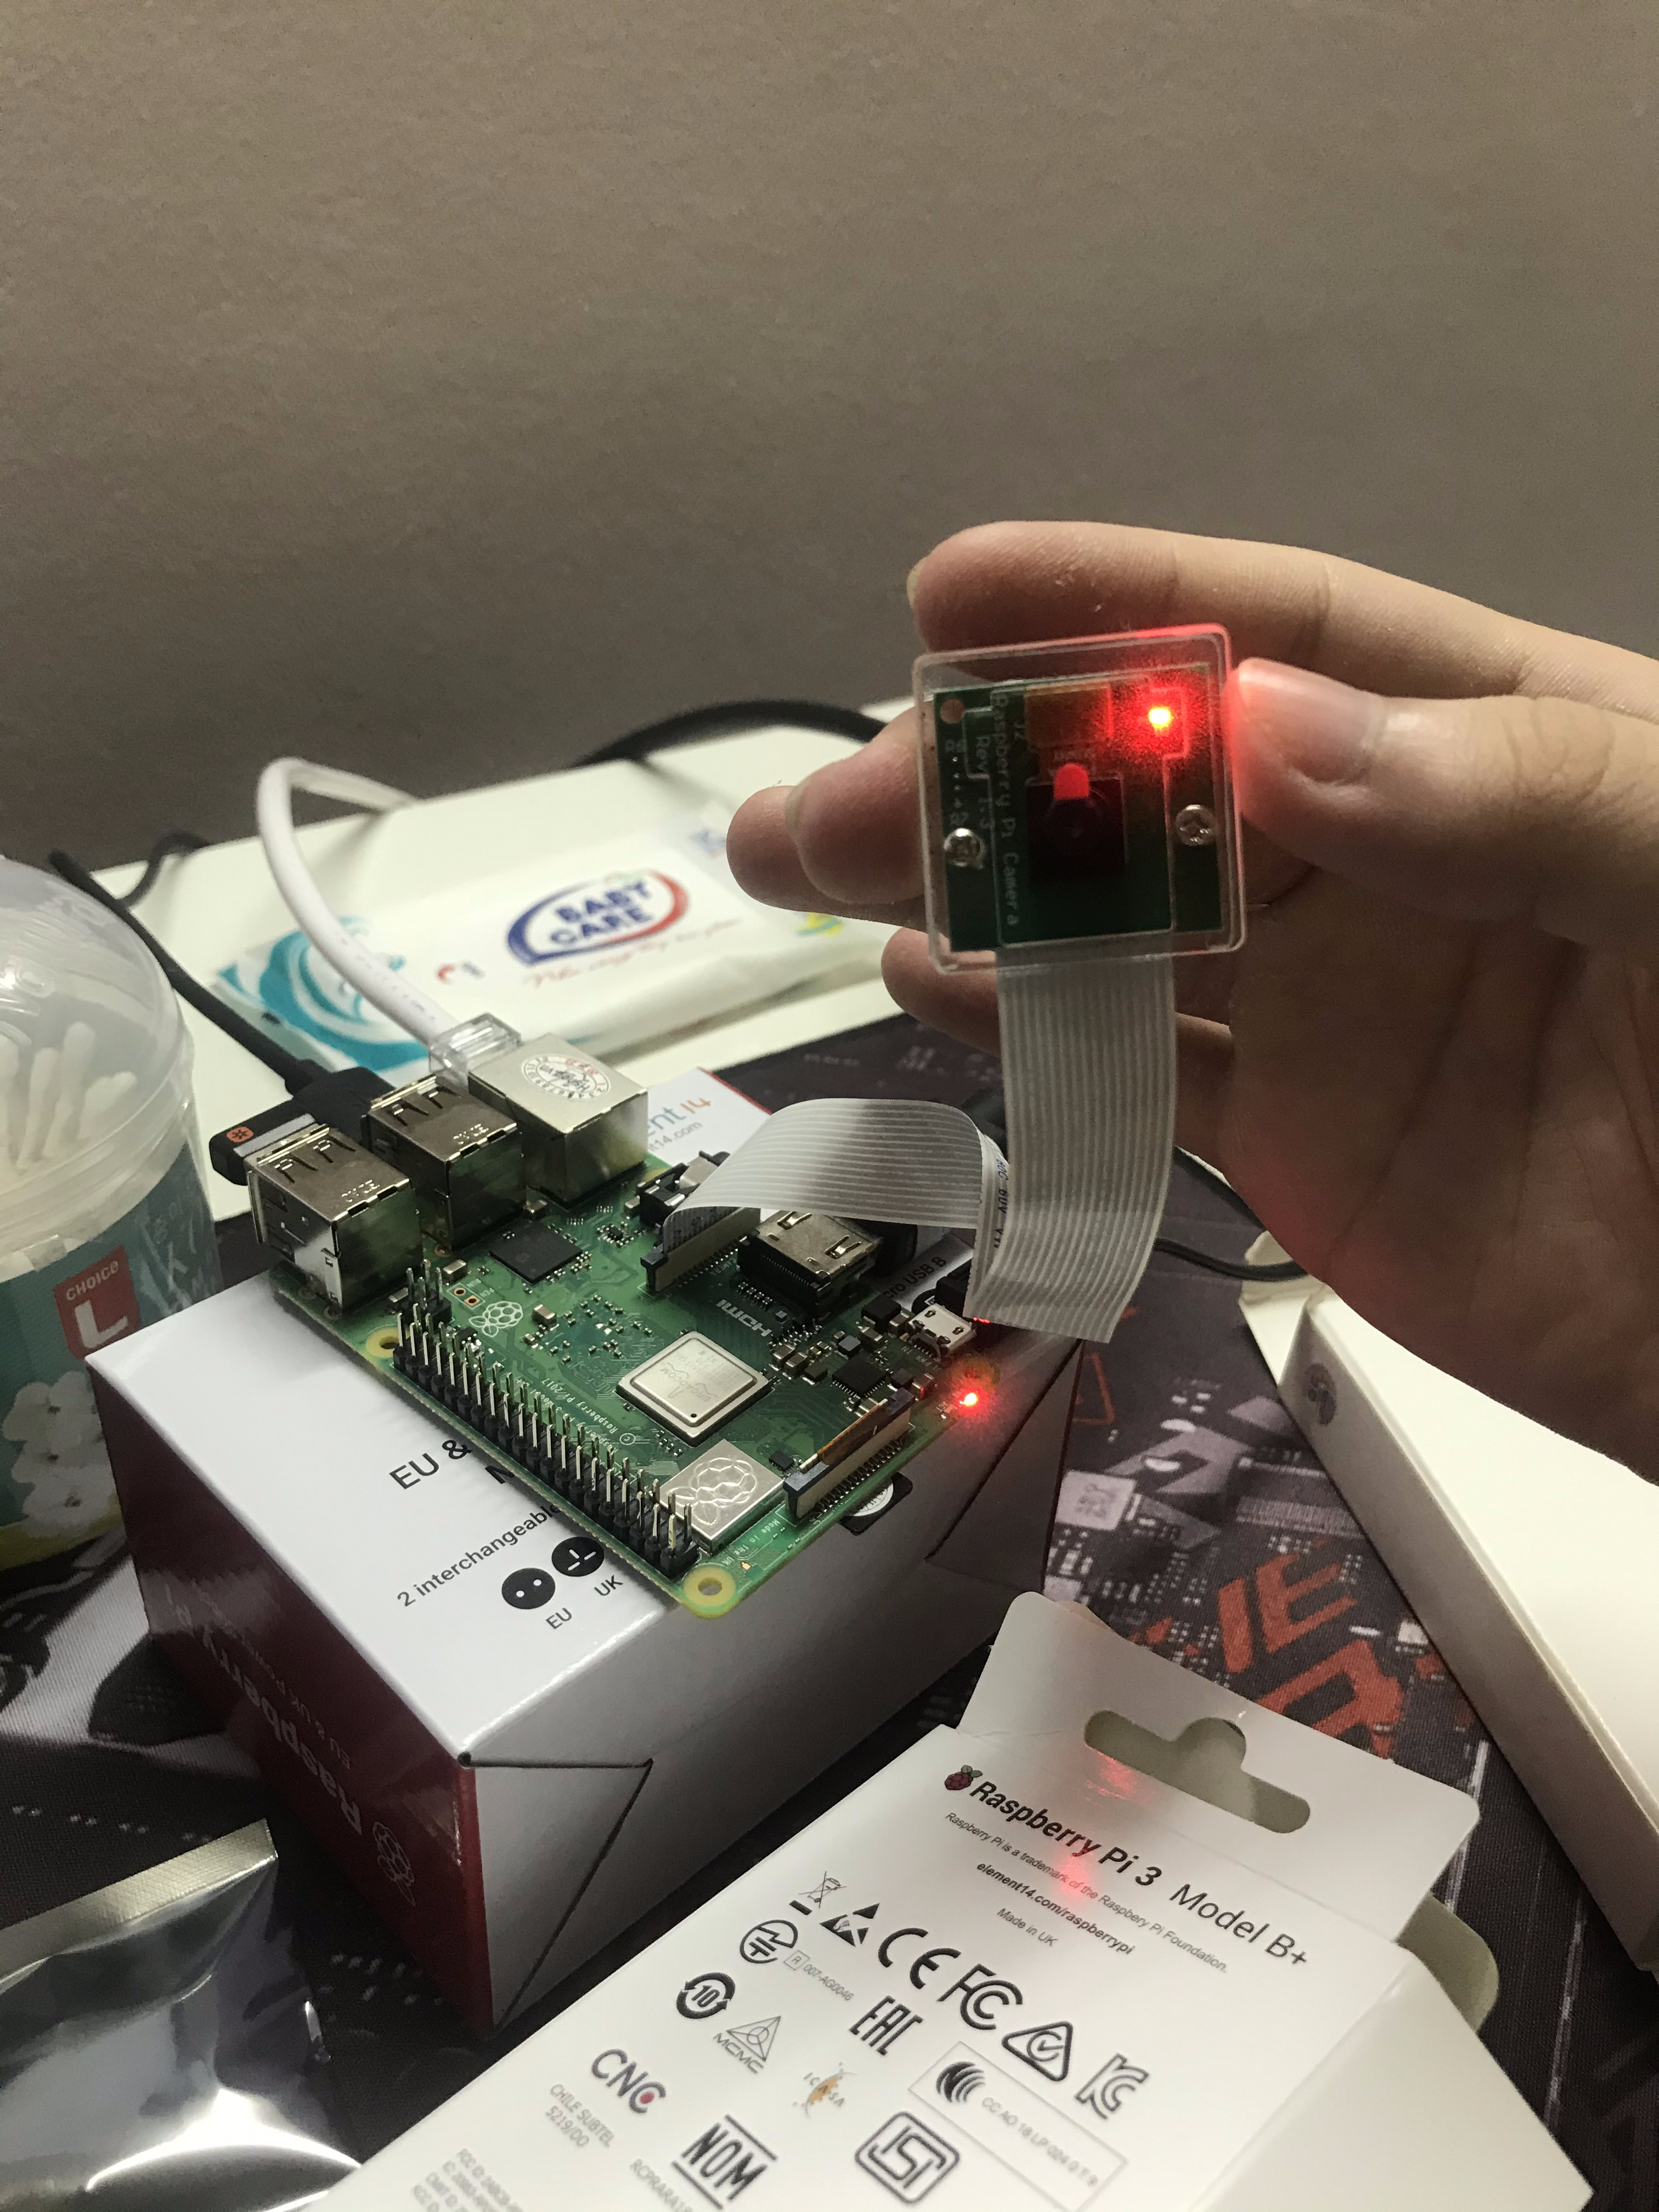
\includegraphics[width=0.6\linewidth]{img/Hardware.png}
        \caption{Drowsiness detection model}
    \end{figure}
\section{Result}
    \begin{figure}[H]
        \centering
        \includegraphics[width=0.6\linewidth]{img/run.png}
        \caption{Eye aspect ratio}
    \end{figure}
    \begin{figure}[H]
        \centering
        \includegraphics[width=0.6\linewidth]{img/result.png}
        \caption{Drowsiness detected}
    \end{figure}

    \chapter{MODEL TRAINING}

\renewcommand{\headrulewidth}{0.5pt}
\renewcommand{\footrulewidth}{0.5pt}
\thispagestyle{plain}
\pagestyle{fancy}
\fancyhf{}
\fancyhead[L]{\textbf{CHAPTER 5}}
\fancyhead[R]{\textbf{Intelligent Traffic System}}
\raggedright
\fancyfoot[L]{From: ITM Vision}
\fancyfoot[R]{Page \thepage}

\section{Dataset}

\section{Loss Function}

\section{Hyperparameters}



\end{document}